\begin{figure}[h]
  \centering
  
%segundo bloco de figuras
  \begin{tabular}{@{}c@{} p{3cm} @{}c@{} }
    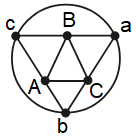
\includegraphics[width=3cm]{./img/octaedro.png} & &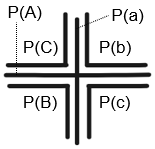
\includegraphics[width=3.5cm]{./img/representacaoOctaedro.png}  \\[\abovecaptionskip]
    \footnotesize (a) The octahedral $O_3$ graph  & &  \footnotesize(b) $B_1$-EPG($O_3$) Representation
  \end{tabular}
%  \vspace{\floatsep}
 % \begin{tabular}{@{}c@{}}
  %  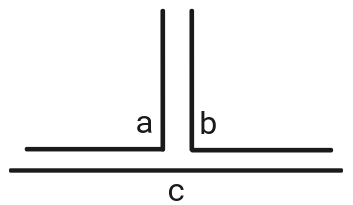
\includegraphics[width=4cm]{./img/b1epgtriangulo.png} \\[\abovecaptionskip]
  %  \small (b) Another image
  %\end{tabular}
 \caption{The octahedral $O_3$ graph and its  $B_1$-EPG representation, \cite{heldt2014}}\label{fig:octaedro}
\end{figure}